%
% requisitos.tex - padsoft 2014
% (c) 2014  M. Blanc, V. Macias
%

% pagina tamaño A4
\documentclass[a4paper, 12pt]{article}

% español
\usepackage[utf8]{inputenc}
\usepackage[spanish]{babel}

% hipervinculos transparentes
\usepackage[colorlinks=true,linkcolor=black,urlcolor=black]{hyperref}

% estilos
\usepackage{enumitem}%{enumerate}
\usepackage{titlesec}
\newcommand{\sectionbreak}{\clearpage}
%\titleformat{\section}{\huge\bfseries}{\thesection}{1em}{}

% elementos matematicos
\usepackage{mathtools}
\usepackage{geometry}
%\geometry{letterpaper} 

% simbolos de euro
%\usepackage[official]{eurosym}
%\usepackage{newunicodechar}
%\newunicodechar{€}{\euro{}}

% diagramas e imagenes
%\usepackage{tikz}
\usepackage{graphicx}


\begin{titlepage}
	\title{Documento de análisis de requisitos}
	\author{M. Blanc \texttt{manuel.blanc@estudiante.uam.es} \and V. Macias \texttt{victor.macias@estudiante.uam.es}}
	\date{Viernes 31 de Enero, 2014}
\end{titlepage}

\begin{document}
	\clearpage\maketitle
	\thispagestyle{empty}
	\tableofcontents

\section{Introducción}

\subsection{Proposito del sistema}
El objetivo del proyecto es analizar, diseñar y programar una aplicacion para la gestion de prestamos de un videoclub. El sistema debe facilitar el control del inventario

\subsection{Ámbito del sistema}
Resumen de lo que el sistema tiene que hacer y qué cosas no tiene que hacer (hasta dónde llega la funcionalidad).
El sistema debe permitir controlar el stock y los prestamos. Además, debe permitir al gestor del videoclub obtener estatisticas sobre los clientes.

\begin{itemize}
	\item Control de desperfectos. No es necesario ya que se efectua a traves de otra via.
	\item Administración de la caja.
\end{itemize}

\subsection{Objetivos y criterios de exito del proyecto}
Los puntos principales son:
\begin{itemize}
	\item Control de desperfectos. No es necesario ya que se efectua a traves de otra via.
	\item Administración de la caja.
\end{itemize}



\subsection{Definiciones, acronimos y abreviaturas}
Un usuario esta definidio como una tupla ordenada
\begin{description}
	\item[UID]      		Identificador unico del usuario (10 digitos)
	\item[Nombre]   		Nombre completo (con apellidos). Deberia ser UTF8.
	\item[DNI]      		Número completo de DNI (con letra), o alternativamente el NIE.
	\item[Direccion]	Dirección completa. \textit{Opcional.}
	\item[Telefono] 		Numero de telefono, movil o fijo. \textit{Opcional.}
	\item[Mail]     		Dirección de correo electronico \textit{Opcional.}
\end{description}

\subsubsection{Peliculas}
Tiene los siguientes atributos:
\begin{description}
	\item[Título] Titulo de la pelicula
	\item[Fecha] Fecha completa de publicación 
	\item[Categorias] Lista de categorias a las que pertenece
	\item[Director] Nombre del director
	\item[Num. ejemplares] Numero de ejemplares \emph{total}.
	\item[Formato] Formato de la pelicula, puede ser DVD o Bluray.
\end{description}

\subsubsection{Series}
Tiene los siguientes atributos:
\begin{description}
	\item[Título] Título completo de la serie.
	\item[Temporada] Número de temporada.
	\item[Categorias] Lista de categorias a las que pertenece.
	\item[Volumen] Número de volumen. 
	\item[Formato] Formato de la serie, puede ser DVD o Bluray.
\end{description}


\subsubsection{Música}
Tiene los siguientes atributos:
\begin{description}
	\item[Título] Título completo del disco.
	\item[Géneros] Generos musicales a los que pertenece el disco.
	\item[Interprete] Lista de interpretes, separada por comas.
	\item[Año] Año de publicacion.
	\item[Formato] Formato del disco, puede ser CD o vinilo.
\end{description}

\section{Descripción del sistema}
\subsection{Requisitos funcionales}
Tipos de usuario y descripción de las funciones que puede realizar cada uno de ellos.

\subsubsection{Tipo de usuario I: Empleado}
Los usuarios principales de la aplicación van a ser los empleados de la tienda. Los empleados son genteempleados de la tienda deben poder:
\begin{itemize}
	\item Dar de alta socios a partir de sus datos.
	\item Efectuar prestamos de peliculas, series y musica.
	\item Vender tarifas planas a socios registrados.
	\item Cambiar la disponibilidad.
\end{itemize}

\subsubsection{Tipo de usuario II: Propietario}
El propietario de la tienda debe poder configurar diversos aspectos de la aplicaciones, tales como:
\begin{itemize}
	\item Establecer los precios de alquiler de todas las categorias
	\item Crear peliculas/series/etc nuevos en la base de datos
	\item Cambiar el numero de unidades de una pelicula disponibles
	\item Cambiar la disponibilidad.
\end{itemize}

\subsection{Requisitos no funcionales}
Descripción de los requisitos no funcionales, categorizados por tipo (rendimiento, fiabilidad, etc).

\section{Casos de uso}
Para ayudarnos a analizar el problema, hemos desarollado casos de uso de la aplicación.
Al tratarse de un sistema interactivo, es irreal pretender considerar todos los casos de uso.
En los siguientes ejemplos puede haber omisiones.

\subsection{Diagrama de casos de uso}
Aqui va un diagrama.

%\begin{tikzpicture}
%	\draw[dotted]
%	   (0,0) node {1st node}
%	-- (4,1) node[rectangle,solid,draw] {2nd node}
%	-- (0,2) node[rectangle,solid,draw] {3rd node}
%	-- cycle;
%\end{tikzpicture}
%\begin{tikzpicture}
%	\draw (-1,0) to[bend left] (1,0);
%	\draw (-1.2,.1) to[bend right] (1.2,.1);
%	\draw[rotate=0] (0,0) ellipse (100pt and 50pt);
%\end{tikzpicture}

\subsection{Descripcion de los casos de uso}
A continuación se detallan tres casos de uso que hemos estimado importantes: un alquiler, una devolución y una acción administrativa. El criterio que hemos seguido es la frecuencia de ocurrencia.

{  %\renewcommand\thesubsection{\thesection. Caso de uso \Roman{subsection}:}

\subsubsection{Alquiler}
\begin{description}[style=nextline]
	\item[Actor primario] Empleado
	\item[Interesados y objetivos] Cliente desea alquilar un artículo.
	\item[Precondiciones] El cliente debe ser socio, no debe tener ningun articulo por devolver y debe abonar la cantidad correspondiente al prestamo que quiere solicitar.
	\item[Garantía de exito (postcondiciones)] El cliente alquila el artículo y el prestamo queda registrado en la aplicación.
	\item[Escenario principal de éxito] \hfill \\
	\begin{enumerate}
		\item El empleado introduce el DNI/NIA del cliente y el UID del artículo.
		\item Se verifica que los datos introducidos sean validos.
		\item Se comprueba que el cliente tenga permiso para hacer el alquiler.
		\item Se calcula y muestra por pantalla el precio del prestamo.
		\item El cliente efectua el pago (en efectivo o con tarjeta).
		\item Se guarda un registro de la transacción y se genera la factura.
	\end{enumerate}
	\item[Extensiones (flujos alternativos)] Escenarios excepcionales
	\item[Requisitos especiales] Lista de requisitos, probablemente no funcionales
	\item[Lista de variaciones de tecnología y datos] Lista de distintas opciones teconologias para la funcionalidad del caso de uso
	\item[Frecuencia de ocurrencia] Estimacion (erronea probablemente)
	\item[Temas abiertos] Cuestiones que estan abiertas y se plantean para resolucion futura, o para considerarse en futuras versiones
\end{description}

\subsubsection{Devolución}
\begin{description}[style=nextline]
	\item[Actor primario] ...
	\item[Interesados y objetivos] ...
	\item[Precondiciones] Situación necesaria para que el caso de uso pueda darse
	\item[Garantía de exito (postcondiciones)] ...
	\item[Escenario principal de éxito] Interacciones del escenario, numeradas
	\item[Extensiones (flujos alternativos)] Escenarios excepcionales
	\item[Requisitos especiales] Lista de requisitos, probablemente no funcionales
	\item[Lista de variaciones de tecnología y datos] Lista de distintas opciones teconologias para la funcionalidad del caso de uso
	\item[Frecuencia de ocurrencia] Estimacion (erronea probablemente)
	\item[Temas abiertos] Cuestiones que estan abiertas y se plantean para resolucion futura, o para considerarse en futuras versiones
\end{description}

\subsubsection{Configuración administrativa}
\begin{description}[style=nextline]
	\item[Actor primario] ...
	\item[Interesados y objetivos] ...
	\item[Precondiciones] Situación necesaria para que el caso de uso pueda darse
	\item[Garantía de exito (postcondiciones)] ...
	\item[Escenario principal de éxito] Interacciones del escenario, numeradas
	\item[Extensiones (flujos alternativos)] Escenarios excepcionales
	\item[Requisitos especiales] Lista de requisitos, probablemente no funcionales
	\item[Lista de variaciones de tecnología y datos] Lista de distintas opciones teconologias para la funcionalidad del caso de uso
	\item[Frecuencia de ocurrencia] Estimacion (erronea probablemente)
	\item[Temas abiertos] Cuestiones que estan abiertas y se plantean para resolucion futura, o para considerarse en futuras versiones
\end{description}

}

\section{Maquetas}
Aqui van unos preciosos dibujicos hechos con NetBeans.\\
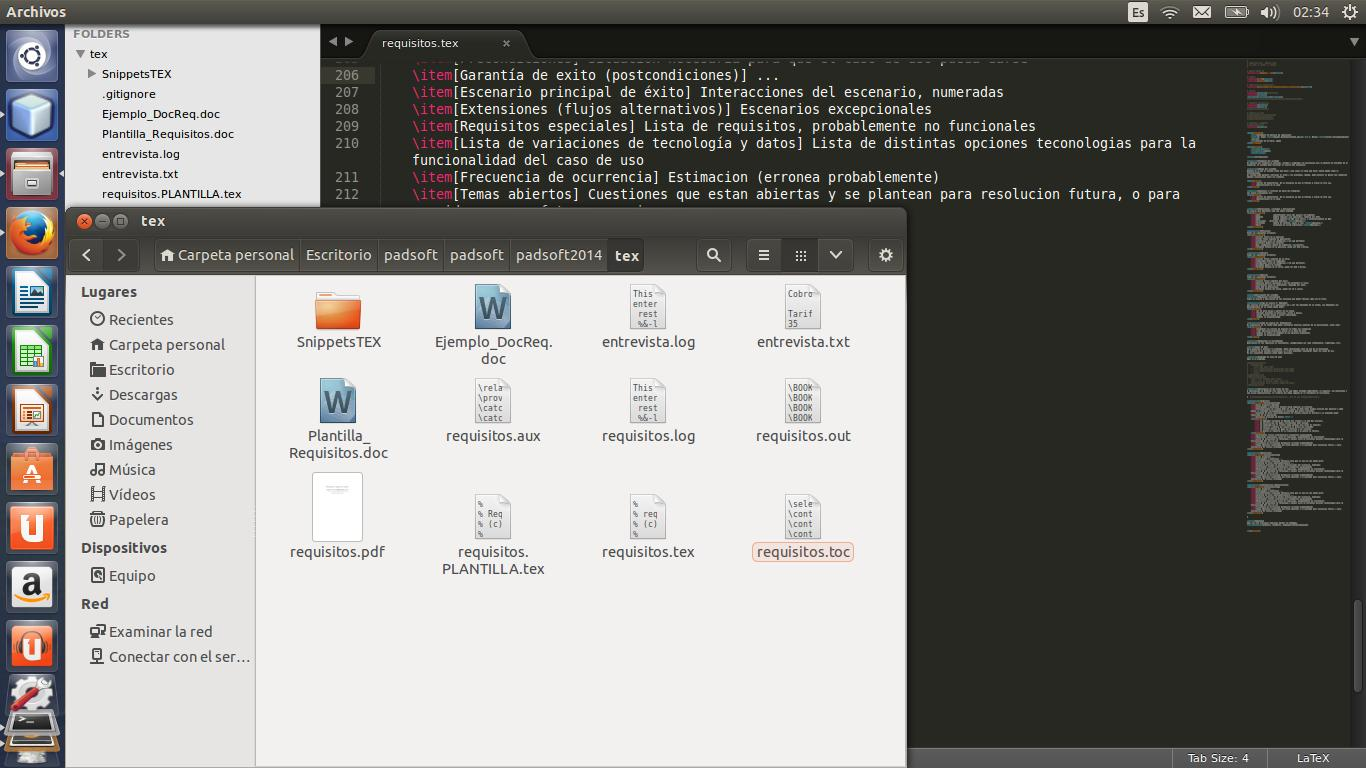
\includegraphics[width=15cm, height=15cm, keepaspectratio]{ZZZ.jpg}
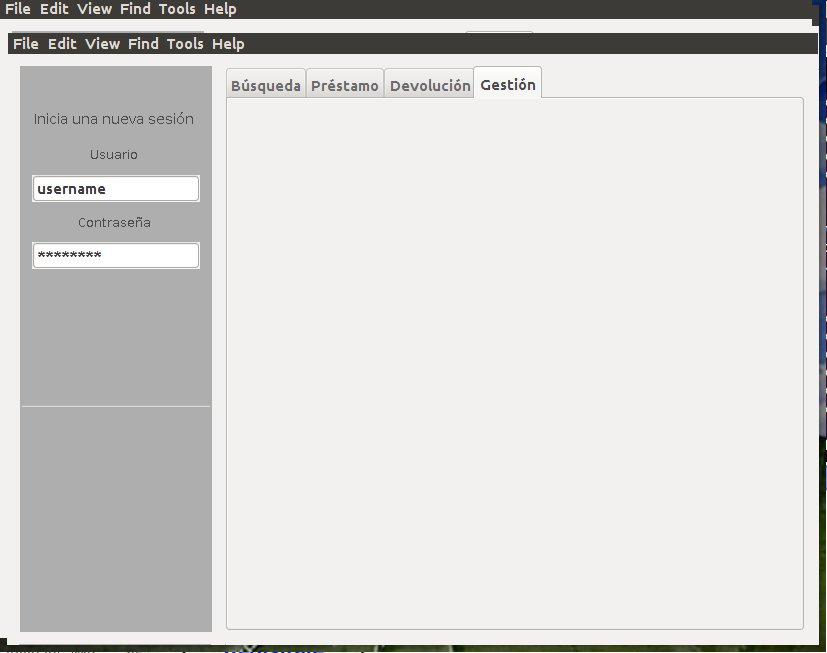
\includegraphics[width=15cm, height=15cm, keepaspectratio]{beta1.jpg}


\end{document}

